\chapter{提案手法の設計と実装}
\label{chap:design_and_impl}
本章では,前提となる Linux カーネルにおけるパケットフォワーディング処理,netfilter に関する知識を解説し,本論文の提案手法についての設計と実装について述べる.

\section{提案手法}
\label{section:proposal-method}
本論文では,netfilter を SR-aware SF として利用するための新しい実装として,Linux のルーティングインフラに netfilter によるパケットのフィルタリングとマングリング機能を統合した End.AN.NF を提案する.
End.AN.NF は,End behavior of SR-aware Native function for NetFilter の略であり,これは SRv6 ビヘイビアの 1 つの種類である.
End.AN.NF は netfilter-based アプリケーションを SR-aware にするのではなく,netfilter そのものを SR-aware にするという考えで設計されている.
これにより既存の netfilter-based アプリケーションは,そのアプリケーションの実装を変更することなく,SRv6 で構築された SFC 環境で SF アプリケーションとして動作させることができる.
End.AN.NF の実装は,Linux カーネルの IPv6 ルーティングスタックを活用するように設計されている.
End.AN.NF の SID は IPv6 アドレスとして表現され,Linux 上では IPv6 のルーティングテーブルエントリとして扱われる.
End.AN.NF を示す SID は,通常の IPv6 経路として既存のルーティングプロトコル,及びその実装を介して他のノードに透過的に広告される.
End.AN.NF は,SRv6 パケットに対して,IPv6 パケットとして netfilter ルールを適用し,かつカプセル化されたインナーパケットに対しても同様に netfilter ルールを適用できる.
End.AN.NF は,nftables\cite{nftables} や iptables~\cite{iptables} などの netfilter-based アプリケーションを介して設定された,トラフィックに対する選択的なパケット破棄や NAT の適用などを SRH でカプセル化された内部のパケットに対しても適用できる.

\section{設計}
\label{section:design}
netfilterは,トランジットするパケットを Linux ネットワークスタックの IPv6 パケット転送フローに既に存在する netfilter フックポイントを通過させ,かつ SRv6 レイヤに 3 つの netfilter フックポイントを持ち,異なるタイミングでパケットに netfilter ルールを適用する.
図\ref*{fig:hooks} は,トランジットパケットに適用される netfilter のフックのフローを示している.
受信したあるパケットに対して End.AN.NF が動作する際,そのパケットは 2 段階の netfilter フックが適用される.
1 段階目の適用では,SRH を含む外部 IPv6 ヘッダのついたカプセル化されたパケットに対して,その外部 IPv6 ヘッダをターゲットにして実行される.
これは End.AN.NF が提供するものではなく,SRv6 パケットが IPv6 パケットとして解釈されて転送される際に適用されるものである.
2つ目の適用では,SRH を含まない,カプセル化された内部パケットの IP ヘッダをターゲットにして実行される.
まず,End.AN.NF カーネルに実装した Linux の SRv6 ノードが IPv6 パケットを受信すると,そのカーネルは受信したパケットに prerouting フックを適用し,通常通り宛先 IPv6 アドレスの最長プレフィックスマッチングを行う.
宛先アドレスが自身の持つ経路表上で End.AN.NF の SID として定義されていた場合,カーネルはパケットを End.AN.NF の実装に渡し,そうでない場合,カーネルは IPv6 レイヤの forward フックと postrouting フックを適用しながら,SRv6 パケットを IPv6 パケットとして解釈し,対応するネクストホップに転送する.
一方,End.AN.NF は,SRH でカプセル化されたインナーパケットに対して,再度,prerouting フック,forward フック,及び postrouting フックを適用する.
この 3 つの netfilter フックポイントは,図~\ref*{fig:nf-hooks} で示されている通り,カーネルがあるパケットをトランジットする際に IP レイヤで通過するフックポイントである.
End.AN.NF の段階で netfilter が適用されている間,SRH は End.AN.NF によって隠されるので,netfilter は SRH の処理を考慮する必要がない.
End.AN.NF が終了すると,外部 IPv6 ヘッダの宛先アドレスは次の SID に置き換えられ,カプセル化されたパケットは Linux の IPv6 パケットフォワーディングプロセスにおける通常の転送パスに戻る.

End.AN.NF は,パケットをマーキングするために SID の \texttt{ARG} フィールドを利用する.
ARG は SID の下位ビットである~\cite{rfc8986}.
SRv6 の仕様上,ある End ビヘイビアがその End ビヘイビア固有の用途で \texttt{ARG} を利用することが許可されている.
End.AN.NF では,SID の \texttt{ARG} がマークとしてカーネル空間におけるパケットバッファに付加される.
netfilter-based アプリケーションは,パケットバッファ上のマーク部分を照合することで,適用するルールを変更することができる.
したがって,オペレータが,単一の End.AN.NF SID しか定義されていない場合であっても,SF アプリケーションは \texttt{ARG} に基づいてトラフィックのルールを調整することが可能である.

アルゴリズム~\ref*{alg:end-an-nf} は,End.AN.NF がパケットを netfilter のフックポイントに渡す方法を示した擬似コードである.
まず,End.AN.NF は,ARG の長さがこの End.AN.NF SID に指定されている場合,受信したパケットの宛先アドレスから ARG 値を抽出する.
抽出された ARG 値は,マークとしてパケットバッファに付加される.
次に,End.AN.NF はパケットバッファの先頭を外側の SRH から内側のパケットに切り替え,バッファを netfilter フックに渡す.
フックにインストールされたルールが内側のパケットに適用された後,End.AN.NF は,パケットバッファの先頭を内側のパケットから外側の SRH に復元し,パケットを次のプロセスに渡す.
この手順は,図~\ref*{fig:hooks} の赤い長方形で示した3つのフックポイント,prerouting,forward,postrouting に対してそれぞれ適用する.

Linux カーネルは,End ビヘイビアを特定の SID を宛先とするルーティングテーブルエントリとして扱う.
End.AN.NF は End ビヘイビアの1つであるため,その SID も同様にルーティングテーブルエントリにインストールされる.
図~\ref*{fig:show-route} に示すように,カーネルは他の End ビヘイビアと同様に End.AN.NF を表す SID をルーティングテーブルエントリとして扱っていることが確認できる.
ルーティングソフトウェアや iproute2 を用いて SID をルーティングテーブルエントリとして追加すると,従来のルーティングプロトコルを用いてカーネルのルーティングテーブルにインストールされた経路を広告することが可能となる.
実際に Linux 用のソフトウェアルータ実装である FRRouting~\cite{frr} を使用し,カーネル内の End.AN.NF に関連付けられた SID を BGP 経由で他のルータに IPv6 経路として広告できることを確認した.
End.AN.NF のアーキテクチャは,ルーティング制御に既存のルーティングプロトコルを使用できるため,既存の SF アプリケーションとの互換性が高い.
このアーキテクチャは,Linux netfilter を用いた SR-aware SF の実現方法の一つである.

\begin{figure}[t]
    \centering
    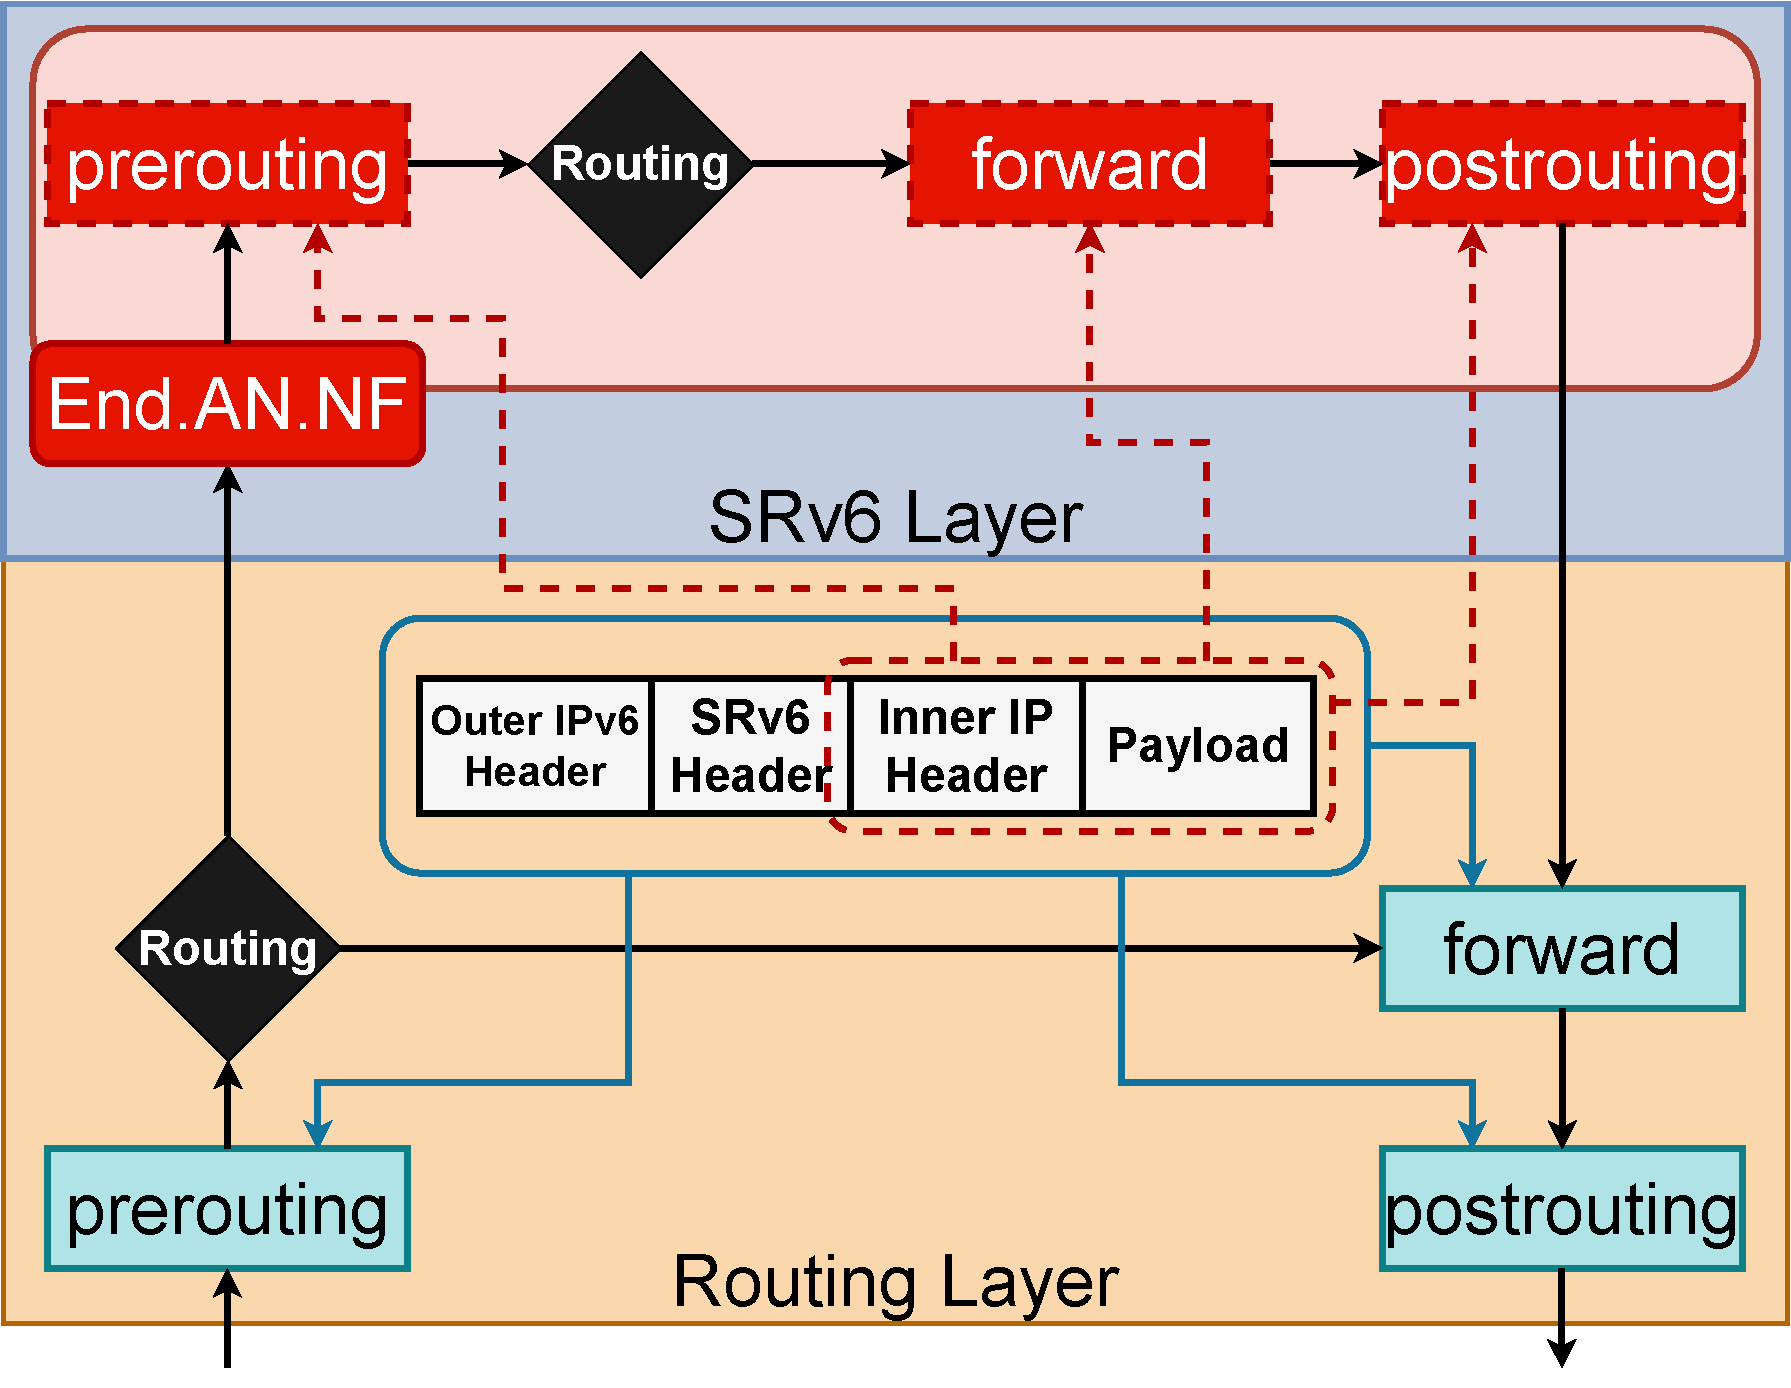
\includegraphics[
      width=0.95\linewidth,
      keepaspectratio=true
    ]{img/End-AN-NF-hooks.pdf}
    \caption{\texttt{End.AN.NF} applies three netfilter hook points, prerouting, forward, and postrouting, to inner packets encapsulated in SRv6.}
    \label{fig:hooks}
  \end{figure}
  
  \begin{algorithm*}[t]
    \caption{Pseudo code of passing a packet to a netfilter hook point in \texttt{End.AN.NF}}
    \small
    \label{alg:end-an-nf}
    \begin{algorithmic}[1]
      \if 0
      \Function {Process\_End.AN.NF}{$packet$}
      \State Call function \textbf{Pass\_to\_Hook} with following args: ($packet$, prerouting)
      \State Decrement segleft by 1
      \State Rewrite destination address based on the SID list and segleft, in the SID of the $packet$
      \State Lookup next hop in th routing table entry for rewrite new destination address
      \State Call function \textbf{Pass\_to\_Hook} with following args: ($packet$, forward)
      \State Call function \textbf{Pass\_to\_Hook} with following args: ($packet$, postrouting)
      \EndFunction
      \fi
      % \Function {Pass\_to\_Hook}{$packet$, $hook\_point$}
      \Function {PassPacketToHook}{$packet$}
      \If {the length of $ARG$ is specified for this \texttt{End.AN.NF} SID}
      \State Extract the $ARG$ value from the destination address of outer SRH
      \State Mark the $ARG$ value on the packet buffer $packet$
      \EndIf
      \State Switch the head of packet buffer $packet$ from the outer SRH to the inner packet
      \State Pass $packet$ to a netfilter hook
      \State Switch the head of packet buffer $packet$ from the inner packet to the outer SRH
      \EndFunction
    \end{algorithmic}
  \end{algorithm*}
  
  \begin{figure*}[t]
    \centering
    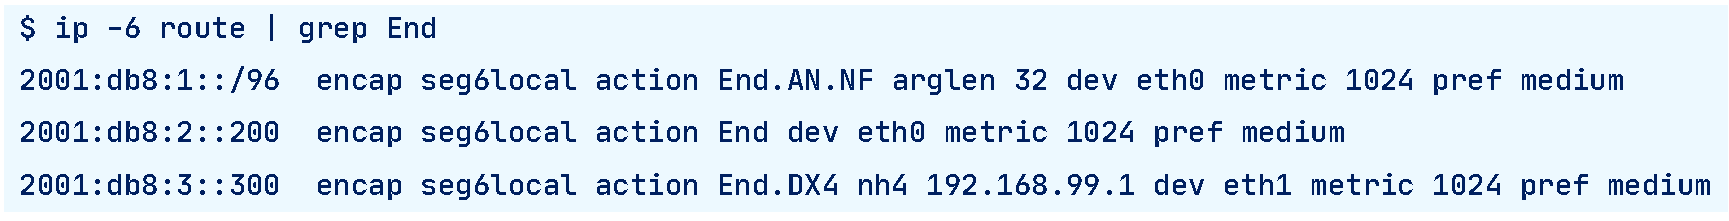
\includegraphics[width=0.95\linewidth]{img/End-FW-show-route.pdf}
    \caption{The modified Linux カーネルtreats an \texttt{End.AN.NF} SID as an IPv6 routing table entry. We can manage the \texttt{End.AN.NF} routes with the existing tools such as iproute2.}
    \label{fig:show-route}
  \end{figure*}

\section{実装}
\label{section:implementation}
End.AN.NF は Linux カーネルで動作する SRv6 ビヘイビアである.
End.AN.NF を実装するためには,Linux カーネルの IPv6 フォワーディングの実装,及び SRv6 の実装を理解する必要がある.
本セクションでは,Linux カーネルにおける SRv6 の実装,及び IPv6 レイヤの netfilter の実装を述べた上で End.AN.NF の実装について説明する.
% Linux カーネルは,End ビヘイビアを関数の SID を宛先とするルーティングテーブルエントリとして実装している.
% このメカニズムは seg6local と呼ばれる.
% End.AN.NF は End ビヘイビアの1つであるため,その実装も seg6local を利用している.
% 図~\ref*{fig:show-route} に示すように,カーネルは他の End ビヘイビアと同様に End.AN.NF を表す SID をルーティングテーブルエントリとして扱っていることが確認できる.
% ルーティングソフトウェアや iproute2 を用いて SID をルーティングテーブルエントリとして追加すると,従来のルーティングプロトコルを用いてカーネルのルーティングテーブルにインストールされた経路を広告することが可能となる.
% 実際に FRRouting~\cite{frr} を使用し,カーネル内の End.AN.NF に関連付けられた SID を BGP 経由で他のルータに IPv6 経路として広告できることを確認した.
% End.AN.NF のアーキテクチャは,ルーティング制御に既存のルーティングプロトコルを使用できるため,既存の NF との互換性が高い.
% このアーキテクチャは,Linux netfilter を用いた SR-aware NF の実現方法の一つである.

\subsection{Linux }
\label{sbsection:linux-packet-forwarding}
